%\documentclass[11pt]{book}
\documentclass[10pt]{article}
%\documentclass[11pt]{amsart}
%\documentclass[preprint,12pt]{elsarticle}
\usepackage{multirow}
\usepackage[all]{xy}
\usepackage{verbatim} 
\usepackage{endnotes}
\usepackage{amssymb} 
\usepackage{setspace} 
%\doublespacing
\onehalfspacing
%\usepackage{mathabx}
\usepackage{amsmath}

%\usepackage{diagrams}

%\usepackage{bookman}
%\usepackage{helvet}
\usepackage{palatino}
%\usepackage{times}


%\usepackage{charter}
%\usepackage{avant}
%\usepackage{chancery}
%\usepackage{utopia}

\def\setgrouptext#1{\gdef\grouptext{#1}}
\newenvironment{groupeditems}{\begin{displaymath}\left.\vbox\bgroup\setgrouptext}{%
  \egroup\right\rbrace\hbox{\grouptext}\end{displaymath}}
  
\usepackage{fancyhdr}

%\pagestyle{fancy}

\usepackage{sectsty}
%\allsectionsfont{\sffamily} 
\chapterfont{\Large \scshape}
\sectionfont{\large \scshape \centering}
\subsectionfont{\normalsize \itshape}
%\subsectionfont{\large \nohang \flushleft} 
%\allsectionsfont{\mdseries\itshape} 
%\sectionfont{\fontfamily{ptm}\selectfont}

% \usepackage{fullpage}


\usepackage[margin=1.5in]{geometry}

\usepackage{lastpage}

\usepackage{fancyhdr}
\setlength{\headheight}{15.2pt}
\pagestyle{fancy}

%\rhead[<even output>]{\textsc{\large Dissertation Summary} --  \thepage \textit{ of}   \pageref{LastPage}}
\rhead[<even output>]{\textsc{\small DRAFT} -- \ \thepage \textit{ of}   \pageref{LastPage}}
%\chead[<even output>]{<odd output>}
\lhead[<even output>]{\text{\small Di Bello \& Verheij}}

%\lfoot[<even output>]{<odd output>}
\cfoot[<even output>]{}
%\rfoot[<even output>]{ \thepage \textit{ of}   \pageref{LastPage}}




\usepackage{pgfplots}

 
\usepackage[round]{natbib}
\begin{document}

\thispagestyle{empty}

\vspace{-2cm}
\noindent
\section*{ \hspace{6cm} \Large DRAFT - begin}
-----------------------------------------------------------------------------------------------------------------------
%\section*{ \Large Writing Sample A}


\vspace{5mm}
\noindent
\textsc{\large \bf  EVIDENTIAL REASONING -- after NYC meeting}

\vspace{3mm}
\noindent
Marcello Di Bello \& Bart Verheij --  \today \\
%Word count:  9723.
\vspace{1cm}

\vspace{1cm}



\vspace{1cm}

%\begin{abstract}
%mmm
%\end{abstract}

%QUESTION: WILL THIS BE A "US CENTRIC" CHAPTER? I HATE THAT, BUT I AM AFRAID MY PART WILL BE US CENTRIC. 

\tableofcontents

\newpage

When a suspect appears in front of a criminal court, there is a very high probability that he will be found guilty. In the Netherlands, for instance, the conviction rate of suspects that appear in criminal courts is reported to be around 95\% year after year.\footnote{Source: CBS, the Dutch central bureau of statistics, publishing its data at www.cbs.nl.} This does not mean that fact-finders deciding about the facts of a criminal case have an easy job. Whether laypeople, such as jury members selected from the general public, or professionals, often experienced judges having completed postgraduate education, all face the difficulties associated with handling the evidence that is presented in court. What to do with conflicting testimonies? Does an established DNA match outweigh the testimony that the suspect was not on the crime scene? How to coherently interpret a large body of evidence? What to do with illegally obtained evidence? When is there enough evidence to convict `beyond a reasonable doubt'? 

The primary aim of this chapter is to explain the nature of evidential reasoning, the characteristic difficulties encountered, and the tools to address these difficulties. There is an extensive scholarly literature on these topics, and it is a secondary aim of the chapter to provide readers the means to find their way in historical and ongoing debates. Before diving into the literature, we set the stage by using two important and often encountered kinds of evidence as an illustration: eyewitness testimony and DNA profiling. Similarities and differences between these kinds of evidence are used to establish a list of central questions and  structure the exposition that follows.

%\subsection{Setting the stage: eyewitness testimony and DNA profiling}

\section{Setting the stage}


Fact-finders, the jurors, judges, or both, aim to reconstruct what has happened in the crime on the basis of the evidence. We will use two types of evidence to develop a list of central questions associated with evidential reasoning: eyewitness testimony and DNA analysis.

\subsection{Eyewitness testimony}

Eyewitness testimony has always been a central source of information in criminal proceedings. It typically takes the form of oral statements by the witness in court, in response to questions by the prosecution, the defense, the court, and sometimes, albeit rarely, the jury. Eyewitness testimony can also come 
in the form of written reports of oral examinations in the pre-court stages of the criminal investigation, normally by prosecuting officers and judges. 

Eyewitness testimony can provide detailed information about what has happened on the scene of the crime. Here is an example.
%
\begin{quote}
Q: Can you describe what happened, that day?

A: I was in the park and suddenly heard a lot of noise, very close by. I saw two men quarreling, shouting. Suddenly one of them pulled a gun, and I heard a shot. The other man fell to the ground. The shooter looked around, looked me in the eye, and then started to run.

Q: Can you describe the shooter?

A: He was a young men, in his twenties, I think. Tall, blonde, with a very white skin, and unusually blue eyes. He looked unhealthy, with bad teeth, like a drug addict. He was wearing an FC Groningen t-shirt, which surprised me as we were in the Vondelpark.
\end{quote}
%
On the basis of eyewitness testimony, we can form a hypothesis about what has happened. Sometimes this hypothesis contains specific detail---as in the example---, still it remains a hypothesis. There are many reasons why the hypothetical events reconstructed on the basis of the testimony may not be true. Typical reasons against the truth of the events reported by an eyewitness include that a witness has wrongly interpreted what he saw, that time has distorted his memories, or that the witness is intentionally lying. 

\subsection{DNA profiling}

DNA profiling has become an important tool in courts. DNA profiling has a strong scientific underpinning, and comes with precise statistical information. The evidential relevance of a DNA profile stems from the fact that, although most of the structure of DNA is shared among all human beings (more than 99\%), the variations that do exist are very specific for each individual. 

A profile is determined by analyzing a number of specific locations---the so-called loci---of a DNA molecule, and establish the type of structure found there. These types are called alleles, and typically consist of the number of repetitions of a small DNA structure at a location. For instance, one locus used in the profiles stored in forensic DNA databases in the USA is referred to as CSF1PO, and it can have alleles 5, 6, 7 and then up to 16, depending on how often the molecular sequence AGAT is repeated at that location.\footnote{See \textit{http://www.cstl.nist.gov/strbase/str\_CSF1PO.htm.}} Different countries use different sets of what are called core loci for their forensic DNA profile databases. For instance, the USA CODIS system has 13 core loci. As said, each specific DNA profile is rare, and reference databases of profiles are used to numerically measure how rare it really is. This is done by counting the number of occurrences of each allele at each core locus in the reference database, which gives an estimate of the proportional frequency of that allele at that locus in the population. The measured proportional frequencies for the individual alleles at the core loci are then multiplied to compute what is called the Random Match Probability of the DNA profile.\footnote{Some special care is needed to accommodate for the fact that an allele can be from either part of the double helix that comprises our DNA.} These Random Match Probabilities---and numbers mathematically related to them---are the numbers reported by forensic experts in courts, and the smaller they are, the higher the evidential value of the profile is taken to be. The sets of core loci have been chosen such that Random Match Probabilities are typically very small, for instance, in the order of 1 in 50 billion, amply exceeding the number of people on our planet. The use of more loci leads to smaller Random Match Probabilities. A key assumption underlying the model is that there are no dependencies among the alleles at different loci. Scientists have found that this is not entirely true, as some dependencies have been established, for instance among the profiles within ethnic groups. It is also accepted that the independence assumption is hard to test in full generality, as that would require assessing more profiles than possible.

Suppose now that a trace of blood has been found on the scene of the crime, and that the found DNA profile matches that of the suspect's DNA. Using this evidence, we form the hypothesis that the suspect is the source of the blood trace, and the Random Match Probability associated with the profile provides a measure of the evidential strength of the match. It is a common misunderstanding to equate this number with the probability that the suspect is not the source of the trace. This well-known misunderstanding is referred to as the prosecutor's fallacy. The probability that the suspect is not the source of the trace can be determined from the Random Match Probability, after a correction for the prior odds that the suspect is the source.

The hypothesis that can be formed on the basis of a DNA match is very specific, and is limited to the suspect being the source of the trace. The hypothesis need not be true, in particular in the cases of an accidental match, the existence of an identical twin---that at a rate of [TO DO: check: 1 in 10000] are not all that rare---, or a lab error. 

\subsection{Central questions}

Using the two kinds of evidence as an illustration, we can now provide the list of central questions associated with evidential reasoning that we use to structure this chapter.

\textit{Question 1:	How should we handle conflicting evidence?}
It often occurs that the evidence provides conflicting perspectives on the crime. For instance, a witness claims that the criminal has blond hair, but the suspect whose DNA matched that of the trace at the crime scene, has dark hair. What to do in case of such conflicts?

\textit{Question 2:	How should we handle the strength of the evidence?}
Some evidence is stronger than other evidence. This is most obvious in the case of DNA evidence, where DNA profiles come with different Random Match Probabilities. But also some eyewitness testimonies are stronger than others. For instance, the description of a criminal by a witness who could only view the crime scene in bad lighting conditions, is of lesser value. How to address the strength of evidence?

\textit{Question 3:	How should we coherently interpret the available evidence?}
A DNA profile match can support that the suspect is the source, and a witness can add information about how the crime was committed. In general, there is a lot of evidence that needs to be coherently combined in order to make sense of what has happened. How do we combine all information in a coherent whole?

\textit{Question 4:	How should we collect, include, exclude evidence?}
During the collection of evidence all kinds of things can happen. An witness' answer to a question can be discarded when the prosecution's question is judged to have lead the witness to an unjustified position. The classic example is the question ``When did you start hitting your wife?'' before it has been established that the suspect has been hitting his wife in the first place. Also DNA material can have been collected illegally, for instance without the suspect's consent. Which rules exist that guide the collection, marshaling, inclusion and exclusion of the evidence?

\textit{Question 5:	How should we decide about the facts given the evidence? When are we done?}
After a careful and exhaustive investigation in the pretrial and trial phases of the criminal proceedings, the question arises when a decision can be made and what that decision is. When is the burden of proof met? What is the meaning of ``beyond a reasonable doubt''? When have we collected enough evidence to make a decision?

In the following sections, each of these questions is addressed. Before that, we discuss three normative tools that can help understand how to correctly handle the evidence.

\section{Three frameworks}

\subsection{Arguments}

\subsection{Scenarios}

\subsection{Probabilities}


\section{Conflicting evidence}

So far we assessed the evidential strength of pieces of evidence considered individually.
When different pieces of evidence are combined, as realistically happens in criminal cases, we might find that they conflict with one another.
For instance, a witness claims that the criminal has blond hair, but the suspect whose DNA matched that of the trace at the crime scene, has dark hair. What to do in case of such conflicts? We first need a general account of how to 
model the \textit{combination} of two pieces of evidence E1 and E2, each supporting, with its own degree of strength, the same hypothesis H. If the strength of a single pieces of 
evidence $E$ depends on how much it impacts $P(H)$, the same applies to 
the combination of two pieces of evidence. 
Bayes' theorem shows us how the combination of E1 and E2 
impacts the probability $P(H)$, as follows:
%
\[\frac{P(H| E1, E2)}{P(\neg H| E1, E2)}=\frac{P(E1\wedge E2|H)}{P(E1\wedge E2|\neg H)}\times \frac{P(H)}{P(\neg H)}.\]
%
If E1 and E2 are independent and do not influence one another, we have:
%
\[\frac{P(H| E1, E2)}{P(\neg H| E1, E2)}=\frac{P(E1|H)}{P(E1|\neg H)}\times\frac{P(E2|H)}{P(E2|\neg H)}\times \frac{P(H)}{P(\neg H)}.\]
%
\[\frac{P(H| E1, E2)}{P(\neg H| E1, E2)}= LR1\times LR2 \times \frac{P(H)}{P(\neg H)}.\]
%
Suppose, in a criminal case, DNA evidence shows that the crime traces match with defendant's 
DNA. The DNA match has a likelihood ratio, relative to hypothesis $S$, of 1,000. Another piece of evidence, independent of the DNA evidence, shows that the crime scene blood type is the same as the defendant's blood type. Suppose the likelihood ratio is now just 10. 
So, the combined evidential strength of the two pieces 
of evidence is $1,000\times 10=10,000$. This is an example of how two pieces of evidence converge  toward the 
same hypothesis.

More generally, two pieces of evidence E1 and E2 are \textit{convergent}, relative to a hypothesis H, whenever they each impact 
upwards the probability $P(H)$, or in other words, whenever their likelihood ratios relative to H are 
both positive, as follows:
%
\[\textsc{Convergence: } LR1=\frac{P(E1| H)}{P(E1|\neg H)}>1 \text{ and } LR2=\frac{P(E2|H)}{P(E2|\neg H)}>1.\]
%
Let's now examine when two pieces of evidence \textit{conflict} with one another. 
[SHOULD WE TALK ABOUT ARGUMENT HERE SOMEWHERE?\footnote{In terms of arguments, if two pieces of evidence conflict, two divergent arguments can be constructed. One will have E1 as its premise and H as its conclusion. The other will have 
E2 as its premise and not-H as its conclusion (or a proposition that entails the negation of H). Indeed, the arguments in question will consist of other premises besides E1 and E2. So, in order to locate the source of the conflict in E1 and E2,  the only difference between the two arguments must be in the premises 
corresponding to E1 and E2.}] In probabilistic terms, the fact that the two pieces of evidence, E1 and E2, are in conflict relative to a hypothesis H can be represented as follows. One piece of evidence E1 raises the probability of H, while the other piece of evidence E2 raises the probability of not-H (or lowers the probability of H). 
So, $P(H)<P(H|E1)$, but $P(H)>P(H|E2)$. In terms of likelihood ratios, this means that
%
\[\textsc{Conflict: } LR1=\frac{P(E1| H)}{P(E1|\neg H)}>1 \text{ and } LR2=\frac{P(E2|H)}{P(E2|\neg H)}<1.\]
%
How can we weight the relative strength of two conflicting pieces of evidence?
Consider an example. At trial, there are two conflicting eyewitness testimonies W1 and W2. One witness asserts that the defendant was around the scene of the crime 
when the crime was committed, abbreviated SC. The other witness offers an alibi for the defendant and asserts that she was with the defendant 
during the time of the crime, abbreviated $\neg SC$.  Suppose SC has a probability of 0.5, regardless of the testimonies W1 or W2.
Suppose, also, that W1 brings the probability of SC to 0.9, whereas W2 brings the probability of H to 0.1 (and thus brings the probability of $\neg SC$ to 0.9). Each testimony has the \textit{same  yet divergent impact} on the probability $P(SC)$. Testimony $W1$ raises the probability of $SC$ while testimony W1 lowers the probability SC. 
They each do so to the same extent but in opposite directions. 
Absent any further information about the trustworthiness of W1 and W2, the two testimonies should cancel one another. 
The evidential strength of each testimony W1 and W2  can be represented, in terms of likelihood ratios, 
as follows:
%
\[LR1=\frac{P(W1| SC)}{P(W1|\neg SC)}=\frac{0.9}{0.1}=9 \text{ and } LR2=\frac{P(W2|SC)}{P(W2|\neg SC)}=\frac{0.1}{0.9}=\frac{1}{9}.\]
%
The combined evidential strength of the two testimonies, $LR1\times LR2=9\times \frac{1}{9}=1$.
When combined, two two testimonies have no impact whatsoever on the probability of SC.
As expected, absent any other information about W1 and W2, the two testimonies 
cancel one another. Their combined evidential strength is therefore null. What should the posterior 
probability $P(SC| W1, W2)$ be? If the combined evidential strength of W1 and W2, is null, then 
$P(SC| W1, W2)=P(SC)$. In our case, $P(SC| W1, W2)=P(SC)=0.5$,  because the value originally assigned to $P(SC)$, 
regardless of the testimonies, was 0.5.



In the British case, R v Adams [1996] 2 Cr App R 467, there was a conflict between DNA evidence and other forms of evidence. The victim was raped and Adam's DNA matched with the traces of semen found on the victim's body. The probability that a random person would match those traces was estimated to be 1 in 200 million. By contrast, the victim gave a description of the perpetrator that did not match Adam's features. Second, when the victim was asked whether Adam raped her, she was unable to identify him. Finally, Adam had an alibi: his girlfriend claimed he was with her during the time of crime. For one thing, DNA evidence suggests Adam's guilt. For the other thing, Adam's alibi, the victim's failure to recognize Adam as the perpetrator, and the fact that Adams did not match the victim's description of the perpetrator, all these pieces of information point toward Adam's innocence. How can we handle conflicting evidence? 

We can propose a simple analysis of the case based on combining likelihood ratios. 
Let;s openly consider the DNS evidence match, call it M; Adam's alibi, call it A; and the hypothesis 
that visited the crime scene, call it SC. As far as the DNA evidence match is concerned, 
the likelihood ratio of interests is as follows:
%
\[LR_M=\frac{P(M| SC)}{P(M| \neg SC)}=200,000,000.\]
%
When it comes to alibi a possible assignment for the like hood ratios is 
as follows:
%
\[LR_A=\frac{P(A| SC)}{P(A| \neg SC)}=\frac{\frac{1}{100}}{\frac{99}{100}} \approx \frac{1}{100}.\]
%
We can see that $LR_A$ is below one, so the alibi doe snot support the hypothesis SC as expected.
The basic idea behind the assignment $LR_A=1/100$ is this. 
Adams's girlfriend would offer an alibi to his boyfriend with a probability of 1 in 100 
even when his boyfriend was in fact not with her. S0, $P(A| \neg SC)=1/100$. This is a low probability. 
The assumption is that Adam's alibi was a good alibi and that Adam's girlfriend was trustworthy. 
If at trial evidence had emerged that Adam's girlfriend was not truth worthy, 
this estimate should be revised downwards. 
(Indeed, these values are somewhat arbitrary, and this is meant to be no more than 
a theoretical exercise.) Further, it is natural to assume $P(A| \neg SC)=99/100$ given that 
Adam's girlfriend would almost always give an alibi for Adam if he 
was not involved in the crime. By combing the two likelihood ratios, we 
get $LR_M\times LR_A=2,000$. The combine likelihood ratio is much lower than 
$LR_M$ but much higher than $LR_A$.

As a matter of fact, Adam was convicted. The jury was persuaded that the strength of DNA evidence 
outweighed the other pieces of evidence. Was the jury justified?










\section{Evidential strength}

A piece of evidence E can support a hypothesis H more or less strongly. 
The evidential strength of E, relative to a hypothesis H, has to do with the extent 
to which E can impact, upwards or downwards, the initial probability of H. The value of the initial probability $P(H)$, 
often improperly called the \textit{prior probability} of H, is determined without 
taking into account evidence E.  The conditional probability $P(H|E)$, often improperly called the \textit{posterior probability} of H, 
takes into account the new evidence E. 
If E raises the probability of H, that is, $P(H|E)>P(H)$, or equivalently the likelihood ratio $\frac{P(E|H)}{P(E\neg H)}>1$, then
E  supports the hypothesis H. 
By contrast, if E does not raise the probability of H, or equivalently the likelihood ratio is equal to or below 1, then 
$E$ does not support $H$.  More precisely, E's evidential strength toward H is
%
\[\textit{\textsc{postitive} iff }  P(H|E)> P(H) \textit{ iff }\frac{P(E|H)}{P(E|\neg H)}>1\]
%
\[\textit{\textsc{null} iff }  P(H|E) = P(H) \textit{ iff } \frac{P(E|H)}{P(E|\neg H)}=1\]
%
\[\textit{\textsc{negative} iff }  P(H|E)< P(H) \textit{ iff } \frac{P(E|H)}{P(E|\neg H)}<1\]
%

The next step is to quantify E's positive evidential strength toward H (and similarly with negative evidential strength).
 There are different approaches in the literature \citep{Fitelson2006}. Here are a couple. We can consider the difference $P(H|E) - P(H)$. The larger the positive difference, the stronger the support which E offers toward H. Alternatively, we can consider the likelihood ratio $\frac{P(E|H)}{P(E| \neg H)}$. The higher the positive likelihood ratio, the stronger the support which E offers toward H. Since it is common to speak of evidential strength in terms 
of likelihood ratios, we shall do the same. 
%
\begin{quote}
\textsc{Measuring evidential strength:} The evidential strength of E relative to H is proportional to 
the likelihood ratio $\frac{P(H|E)}{P(H|\neg E)}$. 
\end{quote}
%
The likelihood ratios is a good measure of evidential strength because it tells how much a piece 
of evidence E can impact the initial probability of a hypothesis H. This can be visualized by means of 
Bayes' theorem:
%
\[\frac{P(H|E)}{P(\neg| H)} = \frac{P(E|H)}{P(E|\neg H)} \times \frac{P(H)}{P(\neg H)}.\]
%
The formulation in terms of prior and posterior odds might appear cumbersome at first, but it is the easiest
formulation as far as calculations are concerned. Even more succinctly,
%
\[\textit{posterior odd} = \textit{LR} \times \textit{prior odds}.\]
%
There is a formula that allows us to derive the posterior probability of a hypothesis H given the new evidence E
from the posterior odds PO, as follows:
 %
\[ \textit{posterior probability of H given E} = \frac{PO}{1+PO}.\]
%
The table below shows how a likelihood ratio of 1,000 can 
impact the prior odds and lead to different values of the 
posterior odds and the posterior 
probability of the hypothesis of interest. 

\vspace{2mm}
\hspace{0.5cm}
\begin{centering}
\begin{tabular}{lcccc}
\hline
Prior Odds & LR  &  Posterior Odds &  $P(H | E)$ \\
\hline
1:10,000 & 1,000 & 1:10 & 0.09  \\
1: 1,000  & 1,000&  1:1 &0.5 \\
1: 100 & 1,000 &  10:1 &  0.909 \\
1: 1 & 1,000 &  1000:1 &  0.999 \\
\hline
\end{tabular}
\end{centering}
\vspace{2mm}

Consider now a criminal case in which DNA evidence agains the defendant is offered. Laboratory analyses show that the defendant matches with the genetic traces 
found at the crime scene. Call this piece of evidence M. The prosecutor's hypothesis is that the defendant is the source of the genetic material found at the crime; call this hypothesis $S$. 
(Note that hypothesis $S$ is not quite the same as the hypothesis that the defendant is guilty. The fact that the defendant is the source of the crimine scene genetic 
material need not entail that he is guilty. He could have left the genetic traces accidentally 
or in a way consistent with his innocence.) What should we conclude about S given M?
How are we to assess the evidential strength of M relative to S?
As said at the beginning, we can identify three major sources of uncertainty 
while drawing inferences from a DNA evidence match:
%
\begin{enumerate}
\item an accidental match
\item a laboratory error
\item a twin brother or a close relative with the same DNA as the defendant 
\end{enumerate}
%
We shall now see how likelihood ratios can represent  
these three uncertainties and assess the evidential strength of a DNA 
evidence match accordingly. 

Let's start with the possibility of a \textit{coincidental match}. Suppose the defendant matches with 
the crime scene DNA; there was no laboratory error; and no close relative has the same DNA. Even under these assumptions, 
the match could still be a pure coincidence. 
This is why DNA evidence matches typically come with a Random Match Probability. 
The RMP expresses the probability that a random person would show a match, so a RMP
conveys information about the possibility of a purely coincidental match.   
The RMP is often an astronomically low value such as 1 in 50 billion. 
When we have DNA evidence matches, it is therefore very unlikely that 
a random person would show a match. The probability of a coincidental match, 
in other words, is typically very low. 

 If we set aside the other two sources of uncertainty, 
the evidential strength of a DNA evidence match, 
whose Random Match Probability equals a probability $p$, is as follows:
%
\[
{ P(S | M) \over P(\neg S | M)} = { 1 \over p}.\footnote{This simple analysis can be found, among others, in \citep{Dawid02} and \citep{Balding2005Weight}.}
\]
%
We put $P(M |S)=1$, that is, given that the defendant is in fact the source, 
the probability of finding a DNA match for him is one. Intuitively, that is true. If the defendant 
actually left the traces, we would expect him to match with the traces. Second, we put $P(M |\neg S)=p$. That is intuitively true, as well. 
The probability $p$ is the value of the RMP, which represents the probability that someones picked at random, namely someone who is \textit{not} 
the source of the crime scene DNA, would match. 
Suppose, in our example, the RMP is estimated to be 1 in 100,000,000. 
The likelihood ratio would be as follows:
%
\[\frac{P(M |S)}{P( M | \neg S )}=\frac{1}{\frac{1}{100,000,000}}=100,000,000.\]
%

Given that the likelihood ratio is such a high number, the DNA match relative to 
hypothesis S has a great deal of evidential strength. 
But, we should not be fooled by the high likelihood ratio. The inference
from the premise `it is unlikely that a random person would match' to 
the conclusion 'it is unlikely that someone who matches is a random person' is wrong. 
The inference is a confusion of $P(M|\neg S)$, which is indeed low, with $P(\neg S | M)$, 
which need not be low at all. This confusion is known in the literature 
as the \textit{inversion fallacy} or the \textit{prosecutor's fallacy} \citep{Thompson1987Interpretation}. 
Bayes' theorem can protect us from this fallacy. By applying the theorem, with different prior odds and a LR=100,000,0000,  
the posterior odds are as follows:

\vspace{2mm}
\hspace{0.5cm}
\begin{centering}
\begin{tabular}{lcccc}
\hline
Prior Odds & Likelihood Ratios  &  Posterior Odds &  $P(S | M)$ \\
\hline
1: 10 million & 100 million & 10 & 0.9  \\
1: 100 million  & 100 million &  1 &0.5 \\
1: 1 billion & 100 million &  0.1 &  0.09 \\
\hline
\end{tabular}
\end{centering}
\vspace{2mm}

Beside a coincidental match, another source of uncertainty with a DNA evidence match is the possibility of a 
\textit{laboratory error}. If the RMP equals 1 in 100,000,000, assigning a likelihood ratio of 100,000,000 rests on two simplifications. 
For one, $P(\text{match}|\neg S)=\frac{1}{100,000,000}$, or more generally $P(M | \neg S)=p$. Intuitively, given a RMP=100,000,000
the probability that someone who is not the source would show as a match is 1 in 100,000,000. This is a simplification because  
the defendant might \textit{not} possess the DNA profile in question, yet laboratory analyses could show that he does
(what is called a \textit{false positive}). To take false positives into account, instead of a match $M$, we should properly speak of a reported match $M_r$. 
A reported match $M_r$ can occur in two situations: when there is a true, factual match $M_t$ or when there is a true, 
factual non-match $\neg M_t$. So, we have:
%
\[
P(M_r | \neg S)= P(M_r | M_t)P(M_t| \neg S) + P( M_r | \neg M_t) P(\neg M_t | \neg S).\footnote{For an explanation, 
see \citep{Thomason2003How-the-Probabi}.}
\]
%
Now, $P(M_t | \neg S)$ equals $p$, and thus $P(\neg M_t | \neg S)$ equals $1-p$.
Also, $P(M_r | \neg M_t)$ describes the laboratory's false positive rate, abbreviated by $FP$.
Finally, $P(M_r | M_t)$ describes the laboratory's true positive rate, or the inverse 
of the laboratory's false negative rate, abbreviated  $FN$. So, we have:
%
\[
P(M | \neg S)= [(1-FN) \times p] + [ FP \times (1- p)].\footnote{See \citep{Thomason2003How-the-Probabi} and \citep{Buckleton2005A-Framework-for}.}
\]
 %
 The formula above shows that in order to properly estimate the value of
 $P(M_r | \neg S)$, we need a statistical estimate of the DNA profile's RMP \textit{as well as} 
 the laboratory's error rates (false positive and negative rates). 
 
The second simplification is $P(M |S)=1$, that is, given that the defendant is in fact the source, 
the probability of finding a DNA match for him is one. This is a simplification because 
the laboratory analyses might fail to show a match even though the defendant did leave 
the traces (what is called a \textit{false negative}). In our new notation, this second 
simplification can be stated as $P(M_r | S)=1$. To take the possibility of a false negative 
into account, we write:
%
\[
P(M_r | S)= P(M_r | M_t)P(M_t| S) + P( M_r | \neg M_t) P(\neg M_t | S).
\]
In the equation, $P(M_t| S)=1$ and $P(\neg M_t | S)=0$. Thus, 
$P(M_r | S)= 1- FN$. 

Putting everything together, a formulation of the likelihood ratio 
that takes into account laboratory errors is as follows:
\[
{P(M_r | S) \over P(M_r | \neg S)} = { 1- FN \over [(1-FN) \times p] + [ FP \times (1- p)]}.
\]
%
Laboratory error rates do impact the likelihood ratio quite dramatically. 
Suppose a DNA profile  has a frequency as low as of 1 in 1 billion. Suppose laboratory false positive 
and false negative rates equal 0.01. If the likelihood ratio is simply equivalent 
to $1/p$, then it would be 1 billion. With the new formulation, we have:
\[
{P(M_r | S) \over P(M_r | \neg S)} = { 1- 0.01 \over [(1-0.01) \times 0.000000001] + [ 0.01 \times (1- 0.000000001)]}\approx 100.\footnote{
The calculation is as follows:

$= { 1- 0.01 \over [(1-0.01) \times 0.000000001] + [ 0.01 \times (1- 0.000000001)]}$

$= { 0.99 \over 0.99 \times 0.000000001 + [ 0.01 \times (0.999999999)]}$

$= { 0.99 \over 0.00000000099 + 0.00999999999}$

$= { 0.99 \over 0.01000000098 }\approx 98 \approx 100$
}
\]
Relatively small error rates can therefore significantly diminish the evidential stregth of a DNA evidence match by dramatically 
reducing the likelihood ratio. In the example, we went from one billion to only one hundred.\footnote{For a  amore systematic discussion of this point, see \cite{Thomason2003How-the-Probabi} who show how even a small margin of laboratory 
error can substantially diminish the probative value of DNA evidence.} 
The impact of laboratory error rates is an indication that no matter how 
low the RMP turns out to be, it will be of relatively little significance when it is unaccompanied 
by an estimate of the laboratory error rates. But the important point here is that the likelihood ratio, as a measure of the strength of the evidence, 
allows us to take this complication into account. 

There is a third source of uncertainty in assessing the evidential strength of a DNA evidence match. There could 
a \textit{twin brother} or a \textit{close relative} who share the same DNA as the defendant.
After all, DNA profiles are not distributed across the population of the earth with a fixed stable probability. It is not the case that each individual has the same probability of been assigned a genetic profile. Rather, DNA profiles are part of our genetic make-up, which we receive through evolution and natural selection. We did not receive our DNA through a random process. Naturally enough, people who are related are more likely to share the same DNA profile than people who are unrelated \citep{Buckleton2005Population, Weir2007rarity}. This is why forensic experts must qualify their statements by saying that the RMP applies to a population of individuals \textit{unrelated to the defendant}. The RMP probability varies depending on the population of interest, Caucasians, African-Americas, Asians etc.  In a court of law, different RMPs are often presented, each relative to a certain reference population. 
There might be variations across different reference populations such as Caucasians, African-Americans, etc.
Importantly, a low RMP will be significantly higher if the reference population is 
that of the defendant's close relatives.  How can we represent this variety of reference 
populations and their impact on the RMP?

HOW CAN WE REPRESENT THIS WITH LR?
SUBPOPULATION EFFECTS?


All in all, likelihood ratios are a promising way for assessing the evidential strength of a DNA 
match relative to a hypothesis of interest, typically the hypothesis that the defendant is the source of the traces. 
Complications aside, if the underlying Random Match Probability is 1 in 10,000,000,  
the likelihood ratio, as a measure of evidential strength, is 10,000,000.
If the RMP is 1 in 1,000,0000, the evidential strength of the 
DNA match would be much lower. The evidential strengths of the two DNA matches can 
be easily compared. As seen earlier, likelihood ratios can also incorporate more subtle information such 
as laboratory error rates.\footnote{Furthermore, likelihood ratios allow for an even more precise statement of the strength 
of DNA evidence toward the proposition that the defendant was the source of the crime traces. 
So far we spoke as though there is such a thing as a genetic match between the defendant's DNA and a the crime trace DNA. 
As a matter of fact, laboratory results do not yield any reported match. Rather, they yield a 
congruence result between two DNA profiles, one from the defendant and one from the crime traces.
The two profiles are never perfectly identical; they are more or less congruent \citep{Kaye1993Dna}. Instead of a reported match, what we really have 
are two pieces of evidence: one is the laboratory test showing that the defendant has the genetic profile $d$ 
and the other is a laboratory test showing that the traces have the genetic profile $t$; call them 
$G_d$ and $G_t$. Instead of $M$, we can use the conjunction $G_d \wedge G_t$. 
The likelihood ratio can therefore written more explicitly as follows:
%
\[
{P(G_d \wedge G_t | S) \over P(G_d \wedge G_t | \neg S)}.
\]
%
This new formulation might not change the actual calculations, but 
it does make the reasoning clearer \citep{Robertson1995DNA-Evidence:-W}.}

The likelihood ratio analysis can be extended to other forms of trace evidence. For example, it can 
be extended to fingerprints: instead of a genetic match, we will have a match 
between fingerprint profiles. The difference with DNA evidence is that we do not have a 
Random Match Probability for fingerprint profiles \citep{Zabell2005Fingerprint-Evi}. Besides fingerprints, the same 
analysis can be used for blood types, glass evidence, and any other type of trace evidence. 
But, again, we do need an estimate of the Random Match Probability 
which we often lack. 


We now turn to \textit{eyewitness testimony}. It will soon become clear 
that, unlike with the case of DNA evidence, we lack the numbers 
to assign probabilities. It is nevertheless useful to see how likelihood ratios can express 
the evidential strength of eyewitness testimonies.  A testimony could be wrong for 
a varieties of reasons, and most notably the following:
%
\begin{enumerate}
\item cognitive error (e.g. perceptual or mnemonic error)
\item lying
\end{enumerate}
%
As a certain fact F happens, the witness should also be able to cognize 
the happening of F. Indeed, the the witness might incur a cognitive 
error, in the form of a misperception or a mistaken memory. Let $C_F$ 
denote the cognitive state in which the witness cognizes F as happening.
The state $C_F$ can denote perception of F or the memory or credence that F has happened.
If F in fact has occurred, the cognitive state $C_F$ 
is veridical, or else $P_F$ is non-veridical and a cognitive error has occurred.
We can easily represented the evidential strength of a cognitive state, relative to a hypothesis F, as follows:
%
\[\frac{P(C_F|F)}{P(C_F|\neg F)}.\]
%
If the cognitive state $C_F$ manifests itself to the subject regardless 
of whether F obtains, the likelihood ratio would be one. The evidential strength of 
$C_F$ would therefore be null. If, instead, the probability that $C_F$ would manifest itself to the subject is 
higher provided that F occurs rather than its negation, $C_F$ would have a positive 
evidential strength relative to F. This is all well and good, but the problem with this analysis is that we cannot directly access cognitive states. In particular, 
we cannot do that in a court of law. Testimonies do not come in the form of 
cognitive states; they come in the form assertions made by witnesses.
Here is where the possibilities of lying and deception come into play.
Although the witness might not be the cognitive $C_F$, she might have an interest in asserting that F 
has occurred anyway. This is lying.

Suppose a witness asserts that $F$ in a court of law, denoted by $A_F$. We are now interested in knowing the 
strength of the evidence $A_F$. This depends on specifying the hypothesis of interest.  
Suppose the hypothesis is that F occurred and the witness did not misremember
nor misperceive, that is, $F\wedge C_F$. The alternative 
hypothesis will be that  F did not occur and the witness did misperceive nor misremember, 
that is, $\neg F \wedge \neg C_F$. The likelihood ratio 
of interest is therefore as follows:
%
\[\frac{P(A_F| F, C_F)}{P( A_F|\neg F, \neg C_F)}=\frac{P(A_F| C_F)}{P(A_F| \neg C_F)}\]
%
The equivalence is based on the idea that $A_F$ immediately depends on whether $C_F$ 
but not on whether $F$. We make assertions depending on our cognitive states, for examples, what we believe or not believe 
or whether we have an interest in lying. Whether a certain fact F occurred does not 
have a direct influence on our assertions (if not indirectly through 
our cognitive states). This, at least, is the assumptions 
about our psychology that justifies the equivalence above. 











DO THE SAME WITH EYEWITNESS EVIDENCE AND LIKELIHOOD RATIOS. POSSIBLE?
ANY NEED OF BAYES NETWORK HERE? USELESS? TOO COMPLICATED?

\section{Coherently interpreting the evidence}

Often criminal cases form a mosaic. A DNA  match can support the hypothesis that the suspect is the source, and a witness can add information about how the crime was committed. There is a lot of evidence that needs to be coherently combined in order to make sense of what has happened. How do we combine all information in a coherent whole? 
Consider a fairly realistic, though still quite simplified, scenario:
%
\begin{quote}
\begin{singlespace}
\textit{Ennio}. A woman is found dead in the woods. The investigators recover remnants 
of semen on her body, which is severely wounded; they also recover blood stains in a parking lot near the woods. 
The blood type matches with victim's blood type and DNA. 
From the semen on the woman's body, a DNA profile is created. 
Forensic experts estimate that the DNA profile in question has a statistical frequency of 1 in 100 million.
Through a database search, it turns out that an individual in the 
neighborhood, Ennio, has a matching DNA profile. Ennio is arrested and 
charged with murder.  
\end{singlespace}
\end{quote}
%
Imagine you are the prosecutor and you are constructing 
an incriminating case against Ennio. To a first rough approximation, four basic 
pieces of evidence are available:
%
\begin{quote}
\begin{singlespace}
(\textit{semen}) Semen traces on the victim's body;

(\textit{blood}) Blood stains in the parking lot;

(\textit{wound}) Wounds from a knife on victim's body;

(\textit{genetic match}) DNA match between Ennio and semen.
%\item[] DNA match between Ennio and some blood steins
\end{singlespace}
\end{quote}
%\noindent
From the prosecutor's point of view,
the four pieces of evidence above tend 
to establish, or at least they make a \textit{prima facie} case in support of 
four hypotheses, as follows:
%
\begin{quote}
\begin{singlespace}

($x_1$-\textit{intercourse}) individual $x_1$ had intercourse with victim;

($x_2$-\textit{fight}) individual $x_2$ had violent fight with victim in parking lot;

($x_3$-\textit{killing}) individual $x_3$ killed victim with a knife;

(Ennio-\textit{source}) Ennio is the source of the crime scene DNA.
%\item[] DNA match between Ennio and some blood steins
\end{singlespace}
\end{quote}
%\noindent
The prosecutor, in constructing his incriminating case, can advance 
the four inferences:

 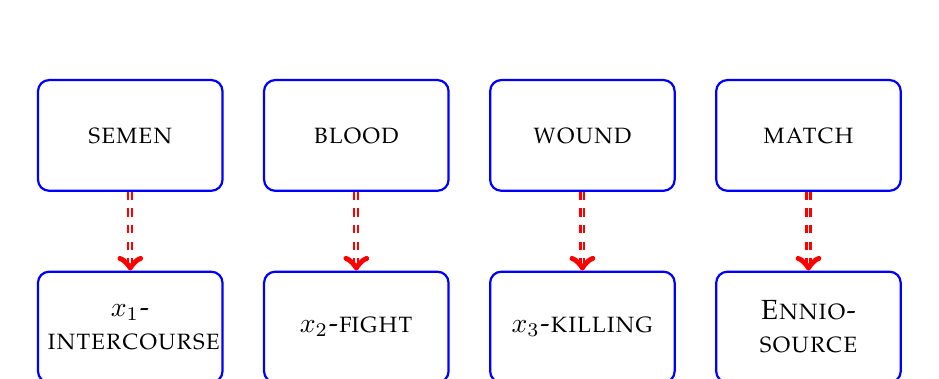
\begin{tikzpicture} 
[auto, 
block/.style ={rectangle, draw=blue, thick, 
text width=6em,align=center, rounded corners, 
minimum height=4em}, 
cloud/.style ={rectangle, draw=red, thick, 
text width=11em,align=center, rounded corners, 
minimum height=4em}, 
line/.style ={draw, thick, -latexÕ,shorten >=2pt}] 
\matrix [column sep=5mm,row sep=10mm] 
{ 
\node [block] (sem) {\textsc{semen}}; 
& 
\node [block] (bl) {\textsc{blood}}; 
&
\node [block] (wo) {\textsc{wound}};
&
\node [block] (ma) {\textsc{match}}; \\ 
% row 2 
 \node [block] (int)  {\textsc{$x_1$-intercourse}}; 
 & 
 \node [block] (f)  {\textsc{$x_2$-fight}}; 
 &  
 \node [block] (kill)  {\textsc{$x_3$-killing}}; 
 &  
\node [block] (pres)  {\textsc{Ennio-source}}; \\ 
}; 
\draw[->, red, double, dashed, thick] (sem) -- (int); 
\draw[->, red, double, dashed, thick] (bl) -- (f); 
\draw[->, red, double, dashed, thick] (wo) -- (kill); 
\draw[->, red, double, dashed, thick] (ma) -- (pres); 
\end{tikzpicture} 

\noindent
The inference from the genetic match to the hypothesis that Ennio is the 
source of the crime scene DNA was discussed earlier while examining 
the evidential strength of DNA evidence.
The acceptability of the other hypotheses
(i.e.\ intercourse; fight; killing) depends on a number 
of case-by-case details: whether the semen on the victim's body was in a quantity, location, 
and arrangement that indicate intercourse; whether the wound on the victim's body was caused by a human artifact, e.g.\ a knife, and whether this caused 
the victim's death; etc. Without dwelling on unnecessary details, let's assume 
that forensic experts, on the basis of their experience, are willing to claim that 
the hypotheses in question can be established, at least \textit{prima facie}  and until 
objections are raised by the defense. 

In order to make a unified case, the prosecutor can advance advance 
a \textit{unification hypothesis}, as follows:
%
\[ x_1=x_2=x_3=\textit{Ennio}\]
%
\noindent
The four initial hypotheses existed in isolation. They still left open the possibility that whoever had intercourse with the victim might be a different person 
from whoever fought with or killed the victim.  They still left open the possibility that different people participated in the crime. 
The unification hypothesis, instead, identifies Ennio as the (only or main) perpetrator. The unification hypothesis, together with the others, asserts that Ennio 
had sexual intercourse with the victim, fought with the victim and finally killed her with a knife. 

We now have a coherent and unifying case against the defendant Ennio.
What is the ground to assert the unification claim? A number of considerations could 
weigh in here: when examined by forensic experts, the crime traces suggest the presence of one perpetrator only; the crime could, in principle, be committed by one person only; Ennio would have had the physical force to commit the crime alone; etc. Depending on the information available, the unification hypothesis will be 
more or less strongly supported. The evidential support for the unification hypothesis cannot be traced back to any single piece of evidence. The support for the unification claim heavily
rests on holistic considerations based on cohesiveness.
Putting everything together, the prosecutor's unified case against 
Ennio can be described as follows:
%
\begin{quote}
\begin{singlespace}
The perpetrator  had or attempted to have sexual intercourse with the victim in the parking lot (which explains the perpetrator's 
semen on the victim's body); a fight ensued during which the victim was wounded (which explains the blood stains in the parking lot); finally, the perpetrator killed the woman with a knife (which explains the wounds on the victim's body) and hid her body in the woods. 
Ennio is the perpetrator: he has a matching DNA profile whose frequency is as low as 1 in 100 millon.
\end{singlespace}
\end{quote}
%

\section{Collection of the evidence and exclusionary rules}

\subsection{Compulsory process}

\subsection{Exclusionary rules}


In general, any relevant evidence is admissible unless it is deemed inadmissible on the basis of 
specific rules of exclusion of which we shall see some examples below.  
%
\begin{quote}
\begin{singlespace}
All relevant evidence is admissible, except as otherwise provided by the Constitution of the United States, by Act of Congress, by these rules, or by other rules prescribed by the Supreme Court pursuant to statutory authority. Evidence which is not relevant is not admissible. (F.R.E.\ 402)
\end{singlespace}
\end{quote}
%
To determine admissibility, it is sufficient to determine whether a piece of evidence is relevant, 
and whether it is deemed inadmissible by some exclusionary rule found in the F.R.E., 
the U.S.\ Constitution, an Act of congress, or rules prescribed by 
the U.S.\ Supreme Court.

Rule 401 of the Federal Rules of Evidence (F.R.E., hereafter) 
defines relevant evidence as follows:
%
\begin{quote}
\begin{singlespace}
Relevant evidence means evidence having any tendency to make the existence of any fact that is of consequence to the determination of the action more probable or less probable than it would be without the evidence. (F.R.E.\ 401)
\end{singlespace}
\end{quote}
%
It is customary to distinguish two dimensions operating in this definition: materiality and probative value \citep{Fisher2008Evidence, Mendez2008}. A piece of evidence $E$ is probative of a fact $F$, provided $E$ makes $F$ more (or less) probable than it would be in absence of $E$. On the other hand, 
a fact $F$ is material for the action or crime $C$ under examination if it is of consequence to the determination of $C$. Whether or not a fact is of consequence to the determination of $C$ depends on the substantive law which determines what facts should be proven in order to establish the crime.\footnote{This is a simplification, however. More precisely, a fact can be material if (a) it is an ultimate issue (one that the governing law says should be proven to establish the crime charged), or (b) it is an intermediary fact, or (c) it is an evidentiary fact. The governing law establishes materiality only for ultimate issues, not for the intermediary and evidentiary facts.} By combining materiality and probative value, it follows that a piece of evidence $E$ is relevant to  crime $C$ if and only if it is probative of $F$, where $F$ is material for $C$.

Once the question of relevance is settled, admissibility becomes a strictly legal question. It depends on the law of the particular jurisdiction. 
For instance, in federal cases, F.R.E.\ 403 establishes that:
%
\begin{quote}
\begin{singlespace}
Although relevant, evidence may be excluded if its probative value is substantially outweighed by the danger of unfair prejudice, confusion of the issues, or misleading the jury, or by considerations of undue delay, waste of time, or needless presentation of cumulative evidence. (F.R.E.\ 403)
\end{singlespace}
\end{quote}
%
Rule 403 requires the judge to perform a balancing test between the probative value of the evidence 
and certain negative or detrimental effects (prejudice, confusions, waste of time, etc.) that 
are more or less likely to occur if the contested piece of evidence is introduced.
Rule 403 is a curious rule, and its standard of application is far from being 
well defined. For instance, what are the items that are intended to be balanced? 
The degree of probative value with the likelihood of prejudice, confusions, waste of time, etc.? 
Or, the degree of probative value with the degree of ``detrimental seriousness''
associated with prejudice, confusion, waste of time? Or does the balancing 
include all three variables? One way to interpret the rule is to say that it requires the judge to compare and balance a purely 
epistemic value---i.e.\ the probative value of a piece of evidence---with other non-epistemic values or dis-values, 
such as prejudice, confusion, and waste of time.\footnote{To be sure, prejudice and confusion might be epistemic (dis)values.} 
The rule states that probative value is not always enough to guarantee admissibility, and hence a balancing test between epistemic and non-epistemic dimensions 
must be performed by the judge. The balancing-test of the two dimensions assumes that they 
can be compared using some common metric. Some have doubted that any balancing test between the two dimensions is possible because it 
would be like comparing apples and oranges, as it were; see \cite{taruffo09}. On the other hand, balancing tests are ubiquitous in the law, especially to reconcile conflicting values and goals. For instance, in 4th Amendment law about (un)reasonable 
searches and seizures two competing goals must be reconciled. One goal is the state's need to collect evidence and the other is the citizen's right not to have their privacy rights violated. The Supreme Court solution, in some cases, is to adopt a balancing-test. It is an interesting question 
whether the ``balancing strategy'' is the only, or the most appropriate strategy to undertake in case of a value conflict.


Another exclusionary rule contained in the F.R.E.\ is rule 404(b), which establishes:
%
\begin{quote}
\begin{singlespace}
Evidence of other crimes, wrongs, or acts is not admissible to prove 
the character of a person in order to show action in conformity therewith.
(F.R.E., 404(b))
\end{singlespace}
\end{quote}
%
Character evidence concerns the previous conduct of the defendant, not the specific conduct 
under examination in the trial. Interestingly, some have recently argued for the relevance 
and admissibility of character evidence \citep{redmayne02}.

HEARSAY EXCLUSIONS


\section{When can we convict?}


%\subsection{Beyond a reasonable doubt}


 What is the meaning of the criminal standard of proof? What does  it take to establish guilt beyond a reasonable doubt? 
  When is a doubt reasonable or unreasonable? Explications of when a doubt is reasonable 
or unreasonable abound. In Commonwealth v.\ Massachusetts Webster (1850), 
proof beyond a reasonable doubt is equated to `reasonable and moral certainty' (295, 59 Mass., 320).  Another paraphrase is that proof beyond a reasonable doubt is such that `a reasonable person would not hesitate to act upon it in the most important of his own affairs,' 
or again, proof beyond a reasonable doubt must cause `an abiding conviction in the minds of the jurors.' These paraphrases might not be that unhelpful, and if so, the U.S.\ Supreme Court is quite right when it says that `attempts to explain the term ``reasonable doubt'' do not result in making it any clearer' (Holland v.\ United States (1954), 348 U.S. 121, 140). Nevertheless, we still have a grasp of what the criminal standard 
is supposed to \textit{do}, though we cannot articulate what it is supposed to \textit{mean}. 
The Supreme Court of Canada in R.\ v.\ Lifchus (1997) listed some platitudes 
about proof beyond a reasonable doubt. They are worth stating:

\begin{quote}
(-) the standard of proof beyond a reasonable 
doubt is inextricably intertwined with that  
principle fundamental to all criminal trials, 
the presumption of innocence;


(-) the burden of proof rests on the prosecution 
throughout the trial and never shifts to the
accused; 

(-) a reasonable doubt is not a doubt based upon 
sympathy or prejudice; 
rather, it is based upon reason and common sense;

(-) it is logically connected to the evidence or  
absence of evidence; 
 
(-) it does not involve proof to an absolute certainty; it is not proof beyond any doubt nor is 
it an imaginary or frivolous doubt;  and

R.\ v.\ Lifchus (1997) at 335.
\end{quote}

\noindent
Most would find the Court's remarks unobjectionable.
The  Court did not only explicate when a doubt is `reasonable,' 
but it also explicitly linked the criminal standard to other related notions, 
such as the presumption of innocence, the burden of proof, the presence and absence of evidence, 
reason and common sense. These connections are important.

In the existing literature, one prominent view is legal probabilism. It is the view that establishing guilt beyond a reasonable doubt means to establish that the defendant's \textit{probability of guilt}, given the total evidence presented at trial, meets a threshold, say, 0.99 or 0.999  \citep{Kaplan1968Decision, Kaye1999Clarifying-the-, Tillers2007}. This definition is simple, crisp and elegant, but a too literal interpretation of it is obviously problematic. Consequently, a doubt would be reasonable or unreasonable depending on a measurable probability.  If a probabilistic threshold is understood as a criterion which the fact-finders should mechanically apply whenever they confront the decision to convict or acquit, two difficulties arise. First, it is not clear where, exactly, the threshold should be placed: is it 0.99, 0.89, 0.899, 0.999, or what? A second difficulty is that assigning a probability value to guilt itself might not be feasible. The second difficuly can be sidestepped if we understand legal probabilism less mechanistically.  The legal probabilists can defend their proposal by conceding that they are not offering a recipe that should be directly implementable in court. Assigning probabilities to propositions, they could say, is an idealized process, a regulative ideal which can improve trial proceedings. In this spirit, setting a probabilistic criterion for criminal convictions would only be a way to theorize about the meaning and function of the criminal standard of proof.

As for the first difficulty---how to identify the threshold---David Kaplan used a relative assessment 
of the disutilities associated with convicting an innocent, $D_i$, and with acquitting a guilty defendant, $D_g$.  
Now, suppose that the probability of guilt 
and innocence equals $P_g$ and $P_i$ such that $P_g = 1 - P_i$. 
To convict---Kaplan suggests---the jury must be believe that 

\vspace{2mm}

$P_g D_g > (1-P_g) D_i$.

\vspace{2mm}
\noindent
The inequality represents a situation in which the expected disutility resulting 
from acquitting a guilty defendant is larger than the disutility resulting from 
convicting an innocent defendant. So, given the inevitable possibility of error, such a situation would be one in which 
convicting is less harmful than acquitting, so that conviction is justified.
But the inequality holds only if $P_g$ reaches a certain value. 
From the above inequality, by algebra, we have

\vspace{2mm}
$\frac{P_g}{1- P_g} > \frac{D_i}{D_g}$.

\vspace{2mm}
\noindent
This formula gives a precise indication of how high the probability 
of guilt must be to justify a guilty verdict, relative to the ratio between $D_i$ and $D_g$. If we consider that
the disutility of convicting an innocent is as harmful as the disutility of acquitting an innocent, 
i.e., $D_g=D_i$---as it might be the case in a civil case---, the lower bound for $P_g$ must be at least $\frac{1} {2}$. 
If, instead,we think that $\frac{D_i}{D_g}=\frac{9}{1}$---as it might be more appropriate in a criminal 
case---, the lower bound for $P_g$ must be at least $0.9$

Some scholars suggested that we should elaborate a 
theory of legal reasoning which departs from the 
probabilistc approach and which does not ignore trial procedures broadly construed
\citep{cohen77, nesson79, Thomson86, Walton2002, Stein05, Pardo2008Judicial-Proof-, ho08, Haack2011Legal-Probabili}.
The key notion here seems to be plausibility rather than probability.
Ronald \cite{Allen2010No-Plausible-Al} recently suggested that that 
`[no] plausible alternative to a plausible story of guilt [should be] the rule of decision in criminal cases'
and that `[i]n criminal cases, fact finders find guilt if there is a plausible story of guilt and 
no plausible story of innocence; otherwise, they find innocence.'

The plausibility-based approach is appealing, but the obvious problem is that the notion of a `plausible story' or of a `plausible alternative to a plausible story' is wholly under-defined. Instead, the theory of probability is well-established and fully worked out mathematically. We should make sure, then, that in abandoning the probabilistic framework, we do not embark into a ill-conceived enterprise. On the other hand, while the notion of plausibility is hard to define precisely, it seems closer to how jurors actually reason in trial proceedings. In contrast, the notion of probability, despite its 
mathematical underpinnings, is hard to relate to actual trial proceedings: jurors do not naturally quantify guilt, and it is difficult to quantify it even if we wanted to. We face a trade-off: probability is a formally developed notion, but it is 
removed from trial proceedings and common-sense reasoning; plausibility lacks a well-established theory, but it is closer to trial practice. 







%\bibliographystyle{spbasic}
\bibliographystyle{plainnat}	
\bibliography{dissertation}






\end{document}

